\section{时序电路}
\subsection{锁存器}
\par 用于存储数据
\begin{figure}[htbp]
	\centering
	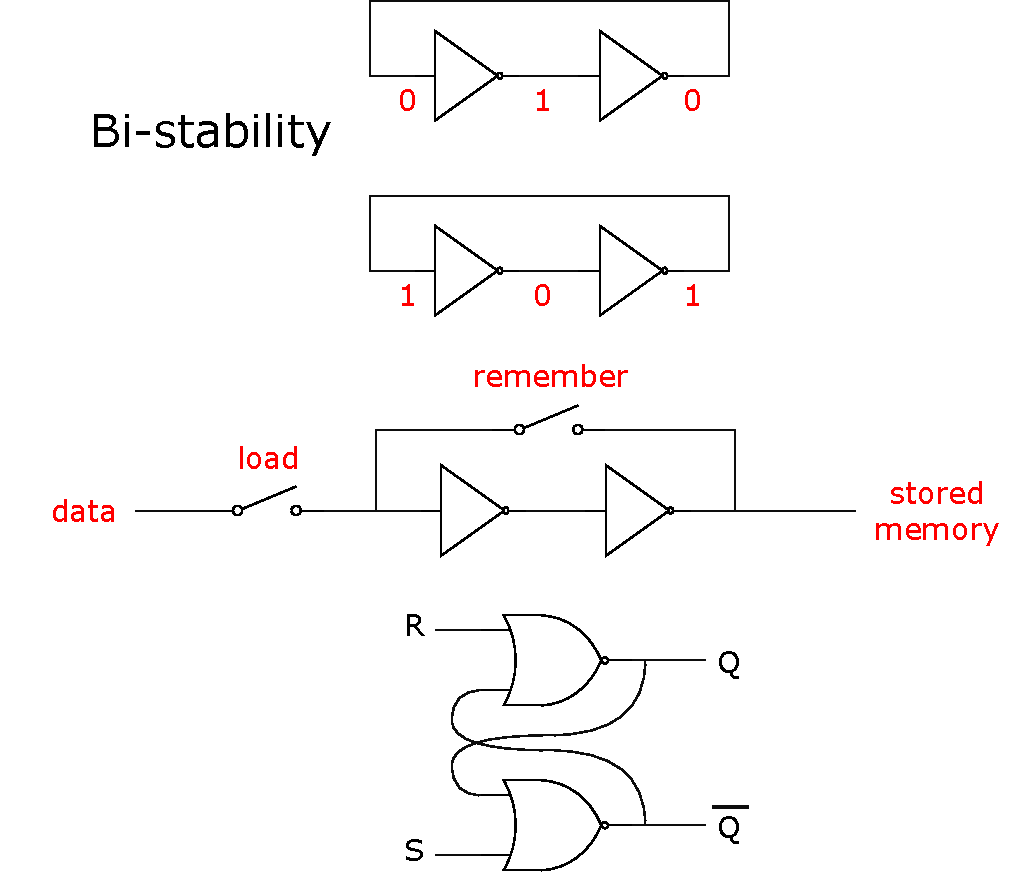
\includegraphics[width=0.6\linewidth]{fig/latches.pdf}
	\caption{SR锁存器(latch)}
\end{figure}
\par SR锁存器状态表
\begin{center}
\begin{tabular}{|c|c|c|c|}
\hline
S & R & 状态\\\hline
0 & 0 & 不变\\\hline
0 & 1 & 复位\\\hline
1 & 0 & 置位\\\hline
1 & 1 & N/A\\\hline
\end{tabular}
\end{center}
\par D锁存器状态:0复位,1置位
\par 门(选通端):决定是否运作

\subsection{触发器}
\subsubsection{SR/D触发器}
\par 触发器状态变化与锁存器相同
\begin{figure}[htbp]
	\centering
	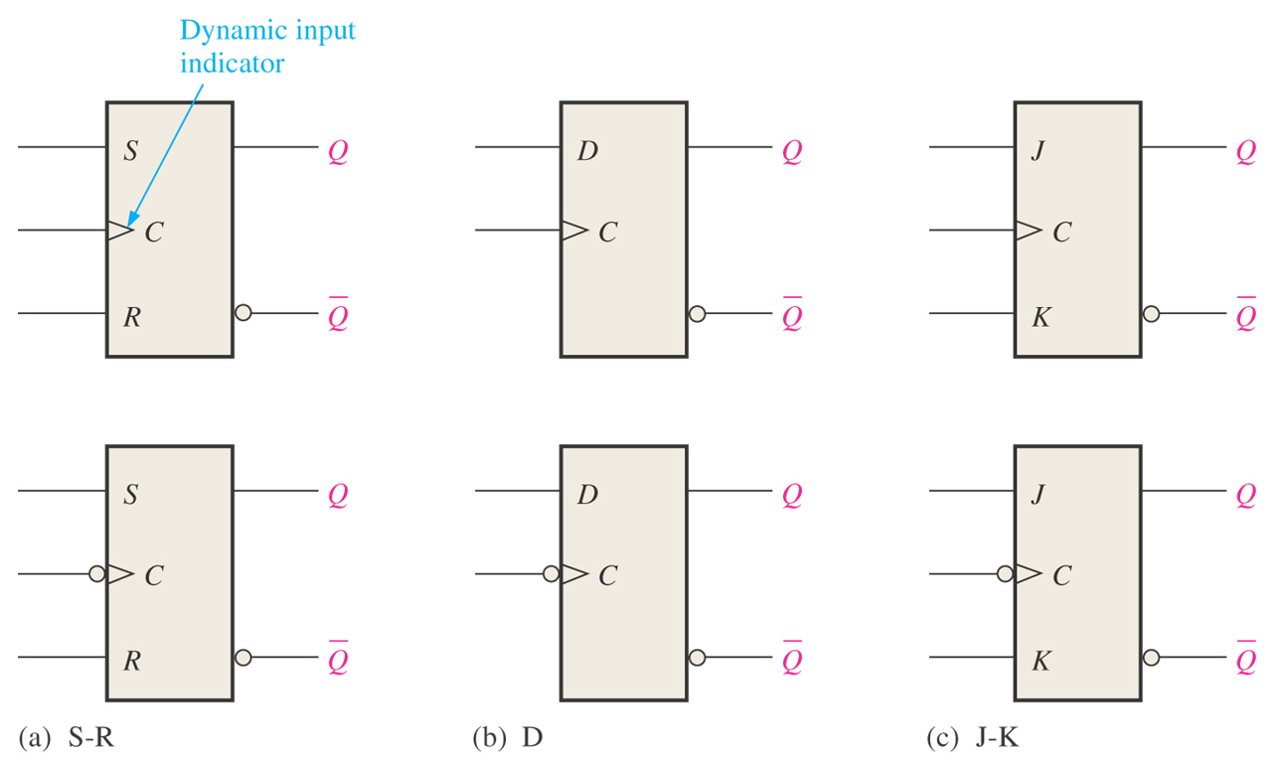
\includegraphics[width=0.6\linewidth]{fig/flip-flops.png}
	\caption{触发器}
\end{figure}
边缘触发其实通过竞争实现(如输入加一个与门后与非$\ol{A\ol{A}}$)
\subsubsection{JK触发器}
\begin{figure}[htbp]
	\centering
	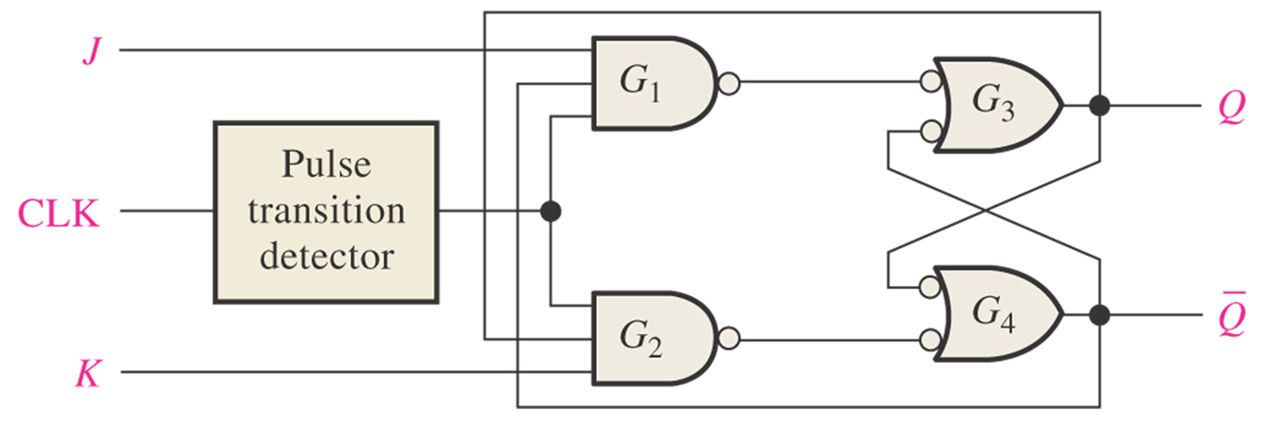
\includegraphics[width=0.6\linewidth]{fig/JK_flip-flop.png}
	\caption{JK触发器}
\end{figure}
\par JK触发器状态表
\begin{center}
\begin{tabular}{|c|c|c|c|}
\hline
J & K & 状态\\\hline
0 & 0 & 不变\\\hline
0 & 1 & 复位\\\hline
1 & 0 & 置位\\\hline
1 & 1 & 转换\\\hline
\end{tabular}
\end{center}
\par 注意看有无\textcolor{red}{bubble},看是上升沿还是下降沿
\subsubsection{应用}
\begin{enumerate}
	\item 并行数据传输:接同一时钟
	\item 分频:JK均接高,遇上升沿才触发,故可实现
\begin{figure}[htbp]
	\centering
	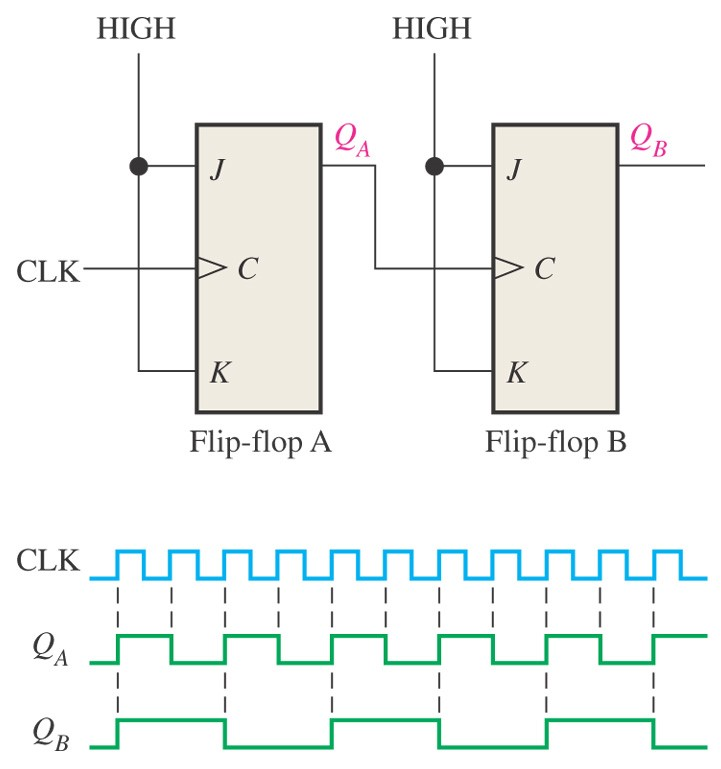
\includegraphics[width=0.4\linewidth]{fig/frequency_divisor.jpg}
	\caption{分频器}
\end{figure}
	\item 计数器:也相当于分频
\begin{figure}[htbp]
	\centering
	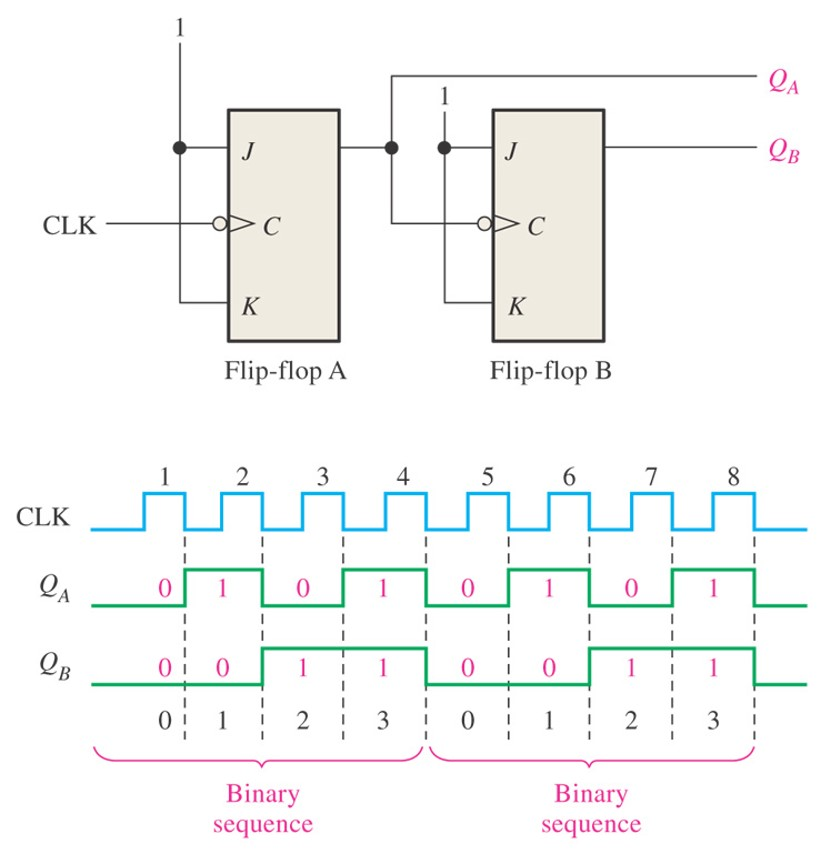
\includegraphics[width=0.4\linewidth]{fig/counter.jpg}
	\caption{计数器}
\end{figure}
\end{enumerate}

\subsection{单稳态触发器}
\begin{figure}[htbp]
	\centering
	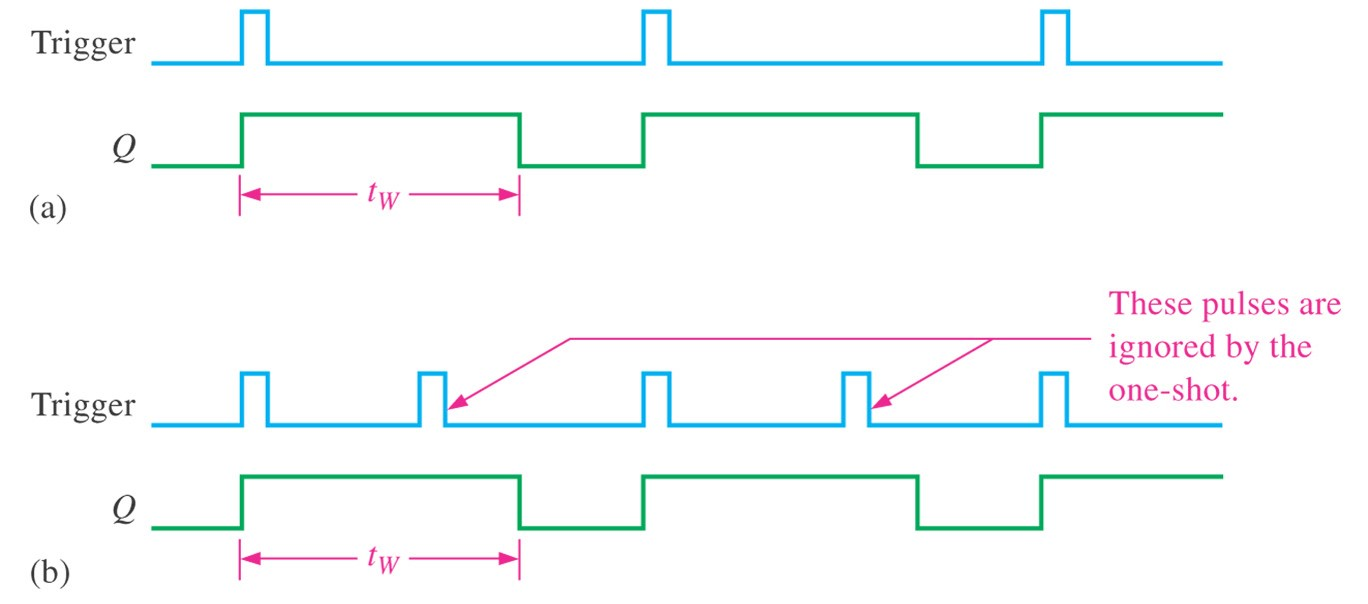
\includegraphics[width=0.6\linewidth]{fig/one-shot.jpg}
	\caption{单稳态触发器(不可重复触发)}
\end{figure}

\subsection{555计时器}
\begin{itemize}
	\item 单稳态触发器(mono-stable one-shot)
	\item 非稳态多谐振荡器(astable multi-vibration oscillator)
\end{itemize}
\begin{figure}[htbp]
	\centering
	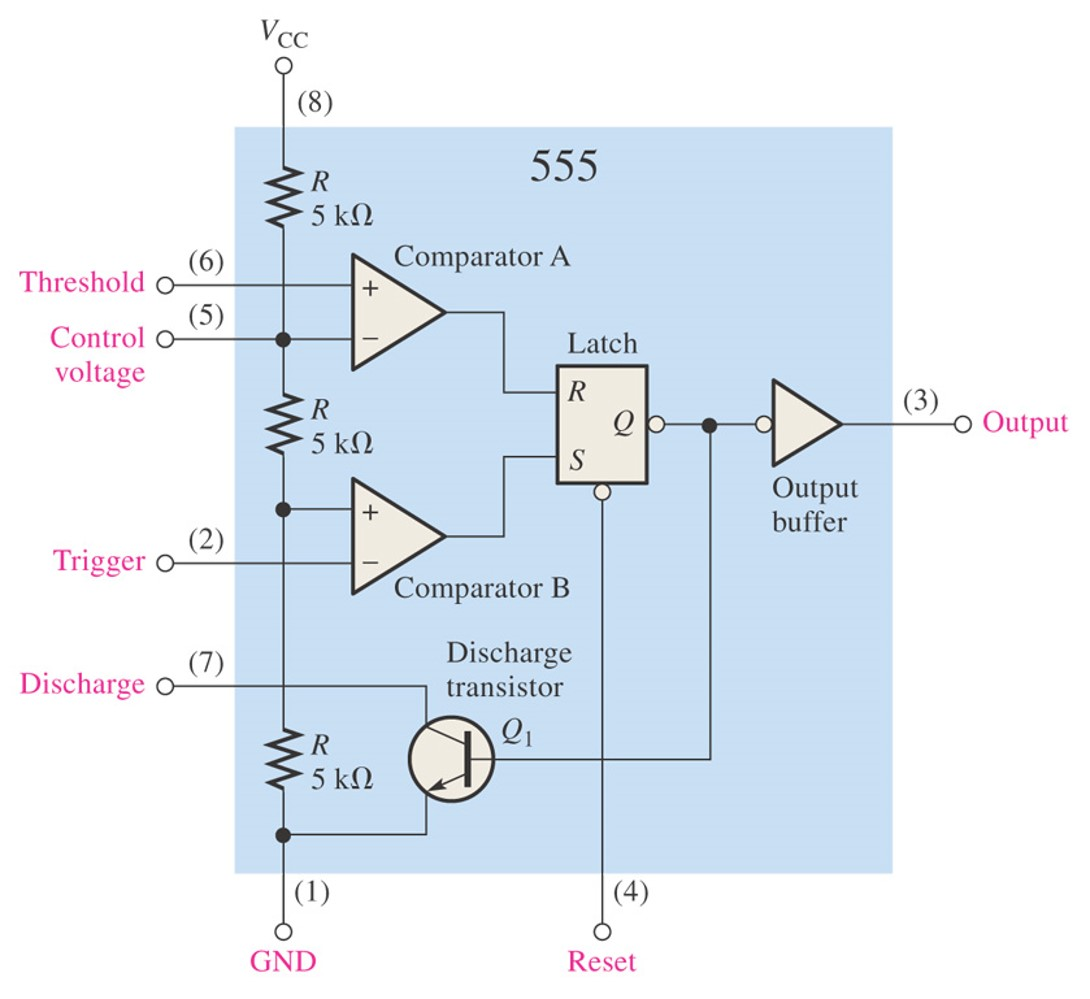
\includegraphics[width=0.6\linewidth]{fig/555timer.jpg}
	\caption{555计时器}
\end{figure}
\[f=\dfrac{1.44}{(R_1+2R_2)C_1}\]
\[DC=\dfrac{R_1+R_2}{R_1+2R_2}\times 100\%\]

\subsection{移位寄存器}
\subsubsection{约翰逊计数器}
\begin{figure}[htbp]
	\centering
	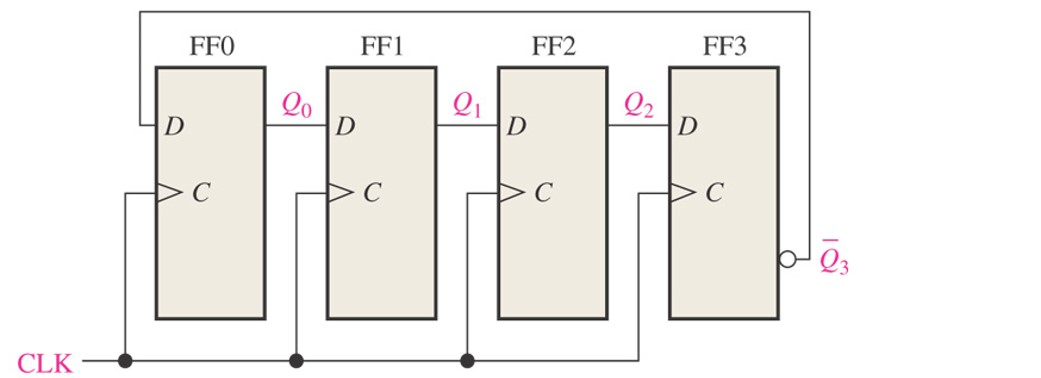
\includegraphics[width=0.6\linewidth]{fig/johnson.jpg}
	\caption{约翰逊(Johnson)计数器}
\end{figure}
\par 计数范围$M=2N$
\begin{center}
\begin{tabular}{|c|c|c|c|c|}
\hline
计数 & $Q_0$ & $Q_1$ & $Q_2$ & $Q_3$\\\hline
0 & 0 & 0 & 0 & 0\\\hline
1 & 1 & 0 & 0 & 0\\\hline
2 & 1 & 1 & 0 & 0\\\hline
3 & 1 & 1 & 1 & 0\\\hline
4 & 1 & 1 & 1 & 1\\\hline
5 & 0 & 1 & 1 & 1\\\hline
6 & 0 & 0 & 1 & 1\\\hline
7 & 0 & 0 & 0 & 1\\\hline
\end{tabular}
\end{center}
\subsubsection{环计数器}
\par 计数范围$M=N$
\begin{figure}[htbp]
	\centering
	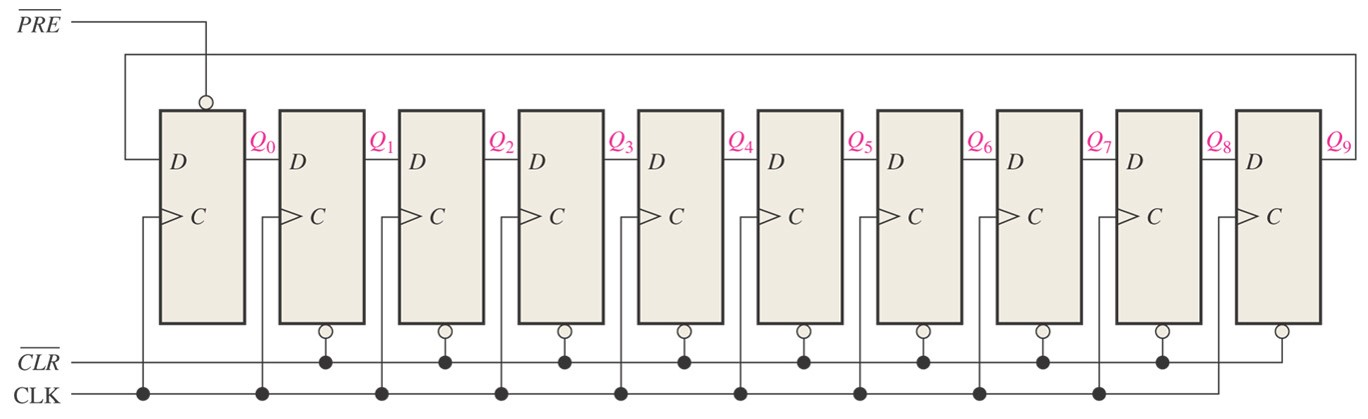
\includegraphics[width=0.6\linewidth]{fig/ring_counter.jpg}
	\caption{环计数器}
\end{figure}
\par 初始置为$1000000000$

\subsection{计数器}
\subsubsection{同步异步计数器}
\begin{figure}[htbp]
	\centering
	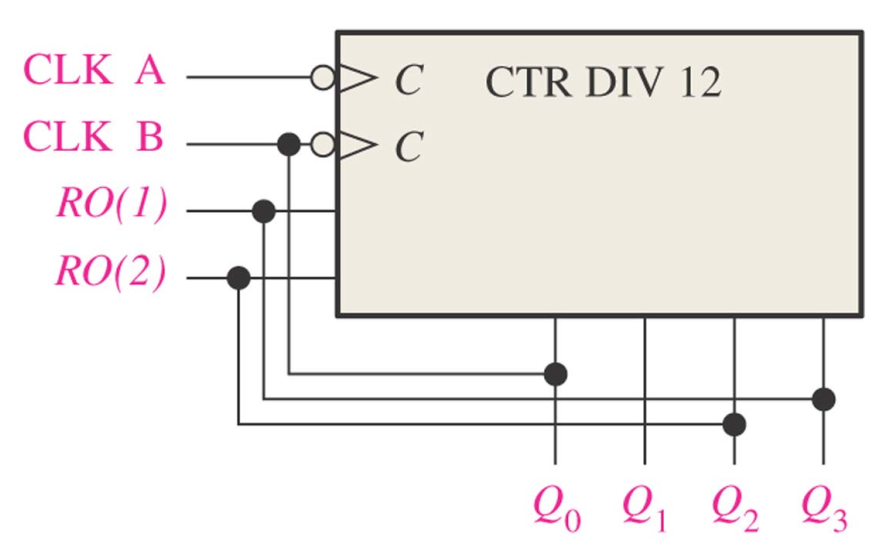
\includegraphics[width=0.3\linewidth]{fig/74ls93.PNG}
	\caption{16进制计数器}
\end{figure}
\par RO(1)与RO(2)同时为高时清零,CLK A控制二进制计数器($Q_0$),CLK B控制八进制计数器($Q_1\thicksim Q_3$),故将$Q_0$输出与八进制计数器相连可得十六进制计数器
\begin{figure}[htbp]
	\centering
	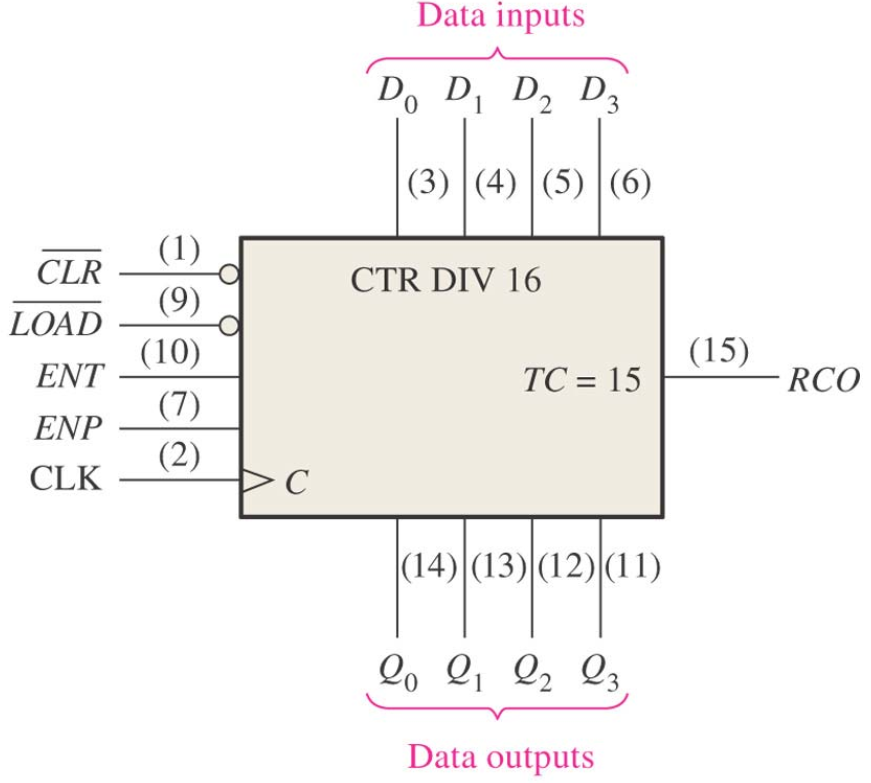
\includegraphics[width=0.3\linewidth]{fig/74hc163.PNG}
	\caption{4位同步二进制计数器}
\end{figure}
\par $\ol{LOAD}$为低时读取数据,ENT、ENP为使能端,同时高电平有效,RCO为进位端
\subsubsection{应用}
\begin{figure}[htbp]
	\centering
	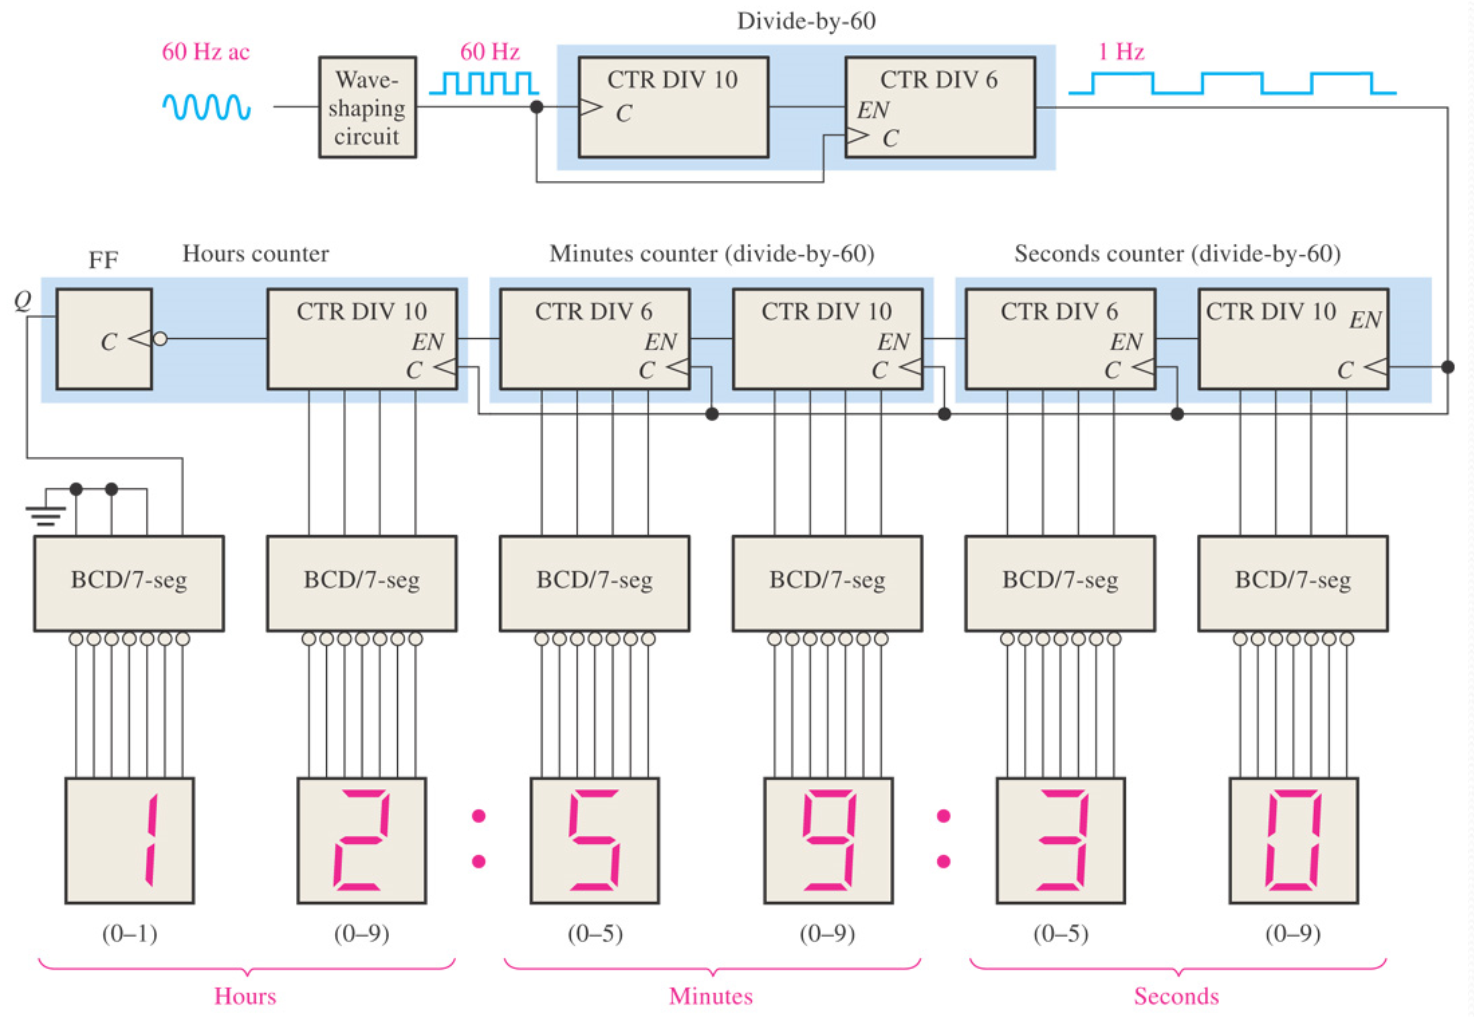
\includegraphics[width=0.6\linewidth]{fig/timer.PNG}
	\caption{时钟}
\end{figure}